\section{Introduction}

\begin{frame}
	\frametitle{Challenge}
	
	\begin{figure}
		\centering
		\begin{tikzpicture}
			\node at (0,0) [draw=white,ultra thick,inner sep=0pt]
			{
				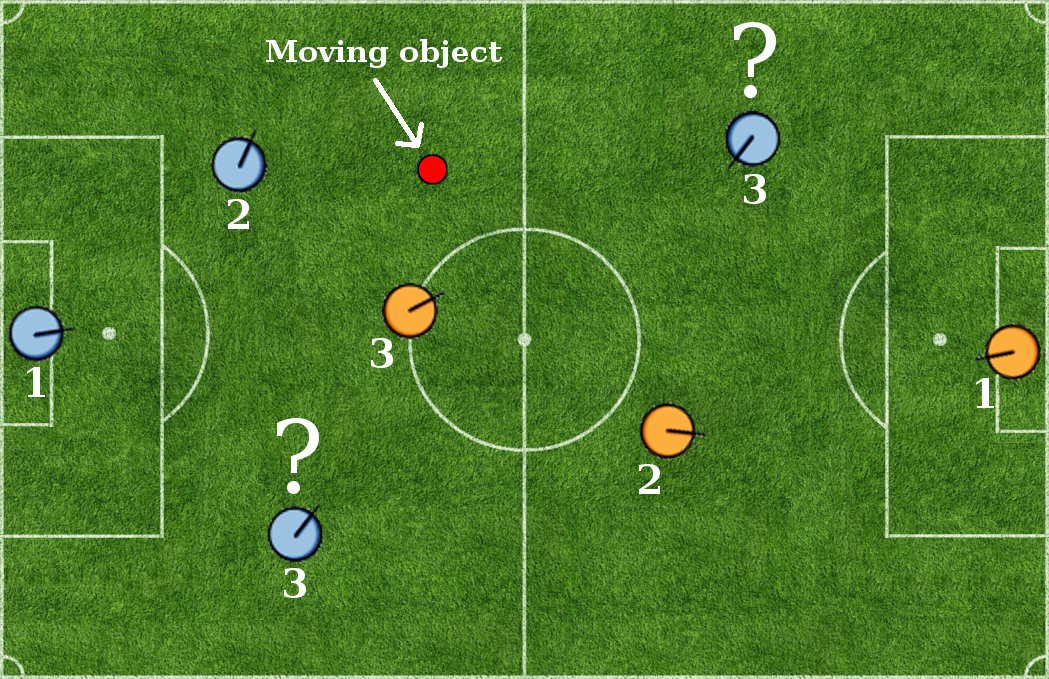
\includegraphics[width=\linewidth]{Figures/Challenge}
			};
		\end{tikzpicture}
	\end{figure}
\end{frame}

\begin{frame}
	\frametitle{Motivation}
	
	\Large
	
	Developing \textbf{distributed applications} using mobile robots is becoming progressively
	more attractive and worthy of investigation, especially in \textbf{video surveillance} \\
	
	\vspace{0.4cm}
	
	Two main research streams arise in this context:
	
	\begin{enumerate}
		\item Distributed decision making
		\item \textbf{Distributed perception}
	\end{enumerate}
\end{frame}

\begin{frame}
	\frametitle{Multi-Object Detection and Tracking}
	\framesubtitle{A brief overview}
	
	\vspace{0.4cm}
	
	\begin{columns}[t]
		\column{0.65\textwidth}
		\centering
		
		\only<1->
		{
			\vspace{0.2cm}
		}
		
		\only<1->
		{
			\begin{block}{Moving Object Detection}
				real-time extraction of moving objects from sensors
			\end{block}
		}
		
		\only<1>
		{
			\vspace{2.84cm}
		}
		
		\vspace{1.0cm}
		
		\only<2>
		{
			\begin{block}{Object Tracking [Yilmaz, 2006]}
				continuous observation of the objects over time to form persistent trajectories of the objects
			\end{block}
		}
		
		\column{0.3\textwidth}
		\centering
		
		\only<1->
		{
			\begin{tikzpicture}
				\node at (0,0) [draw=black,ultra thick,inner sep=0pt]  {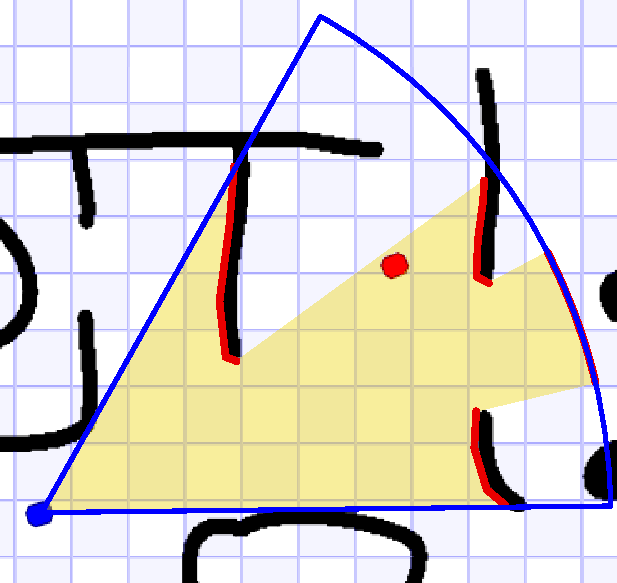
\includegraphics[scale=0.25]{Figures/Agent}};
			\end{tikzpicture}
		}
		
		\vspace{0.5cm}
		
		\only<2>
		{
			\begin{tikzpicture}
				\node at (0,0) [draw=black,ultra thick,inner sep=0pt] {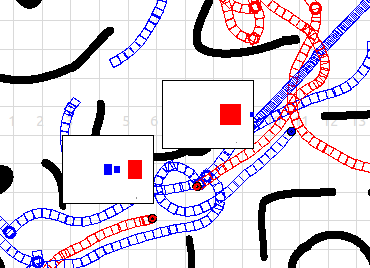
\includegraphics[scale=0.25]{Figures/Stage.png}};
			\end{tikzpicture}
		}
	\end{columns}
	
	\only<1>{\vspace{6cm}}
	\only<2>{\vspace{4cm}}
\end{frame}

\begin{frame}
	\frametitle{Proposed Approach}
	
	\Large
	
	\vspace{0.25cm}
	
	We present a method, called \textbf{PTracking}, based on a novel approach of
	\emph{Distributed Particle Filtering}
	
	\vspace{0.2cm}
	
	The novelties are:
	\vspace{-0.1cm}
	
	\begin{itemize}
		\item Clustering method to track a \textbf{variable unknown number} of objects ensuring
			  a \textbf{limited distribution} in the space
		\vspace{0.1cm}
		\item Approximation of the particle distribution as GMM to improve robustness and
			  reduce network overload
		\vspace{0.1cm}
		\item \textbf{Asynchronous approach} to improve flexibility and robustness of the
			  entire system
	\end{itemize}
\end{frame}
